\chapter{approach}
	This section is the main part of this paper. It illustrates how we formulate the problem we want to solve and what technical skill we use.
	\section{Dataset}
	The main data source of our research is from the Stack Exchange data dump of  1st Sep. 2017 [1]. As all the duplicate pairs have been manually marked by experts on Stack Overflow, we can collect 0.31 million duplicate question pairs. In addition, we can generate as many non-duplicate question pairs as we want.  \par
	We randomly divide the duplicate question pairs into three groups that 80\% for training, 10\% for validation and 10\% for testing. The 80\% subset is mix up with 0.15 million non-duplicate pairs for training the DSSM model, the first 10\% subset is used for validation, and the last 10\% subset is used for the comparison process between our approach and the baselines. 
	
	\section{Overall Architecture}
	We consider the problem as a binary prediction one. Considering an input unit including a well-written title and a list of well-chosen tags, our approach uses the tags to filtering candidates and uses the title to predict and rank those candidates. The main architecture of the DSSM is illustrated in Figure 3.1. \par
	
	\begin{figure}[!h]
		\centering
		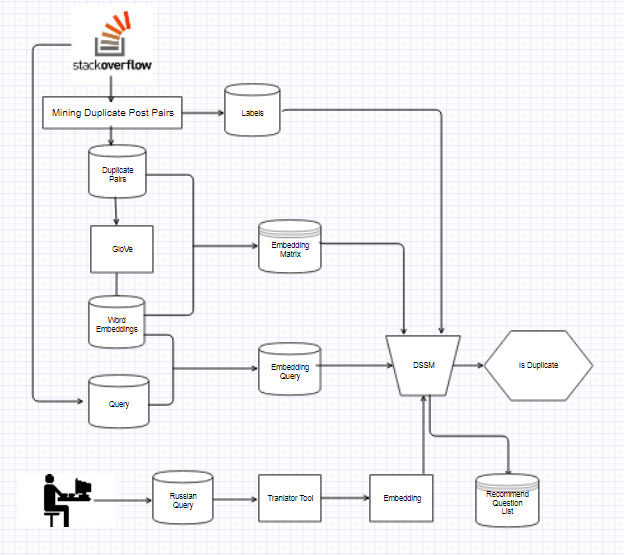
\includegraphics[width = 0.85\textwidth]{figures/model.png}
		\caption{Overview of the Main architecture}
	\end{figure}
	First of all, what we need to do in Step 1 is mining the duplicate question pairs from the raw data of Stack Overflow [1], using the duplicate mark in the Post History file can generate about 310,000 pairs of duplicate questions. We extract the titles and tags of these posts.  Step 2, use GloVe in the process of word embedding and represent all question sentences in vectors after tokenizing them. Step 3, assembling the embedding matrix, which is used for calculating the Weight. Step 4, building the deep learning model. Concatenating the duplicate question pair as input and get a binary variable $is\_duplicate$ as output. In the dense layer. Step 5, training the model and record the best performance from the callbacks. Finally, we get the model that can be used in the recommendation system.
	\section{Learning Word Representation }
	Mapping all the words into a dense low-dimensional vector space, words that appear in the similar sentence have a short distance in the embedding space, and each dimension represents a latent semantic [10,11]. The assumption is that words appeared in the similar context have similar meanings, so their mapped vectors in the embedding vector space should be relatively close. Word embedding only needs a large amount of text to learn as it is an unsupervised method. 
	\par 
	In this paper, we use the Keras tokenizer to tokenize all the questions in the training data set that we mined from the raw data. We also adopt GloVe, which is a popular word embedding tool. For the embedding space, each dimension represents a latent semantic feature of a word. We get a dictionary of all the word that appeared in the text, and finally, there are 0.21 million dimensions in the embedding space. 
	\par
	For example, given an English duplicate question pairs, the word embedding system will convert it into embedding space by mapping each word with the dictionary of words after preprocessing.  Then, concatenating the two vectors as a unit, it will be the input of the deep learning model.
	
	\section{Model Training}
	Figure 3.2 presents the architecture of our deep semantic similarity model(DSSM), which is based on the Stanford Natural Language Inference [12]. This model takes a vector pair of embedded questions as input. Firstly, tokenize the two questions into word sequence then process the word embedding. We need to add padded dimensions to keep all embedding sentences in the same shape (assume each sentence vector has 25 dimensions). Also, we use the GloVe the form a Weight matrix Rw t*Dw that t is the total words number and Dw is the max dimension number of the embedding (assume Dw is 300). 
	\par
	\begin{figure}[!h]
		\centering
		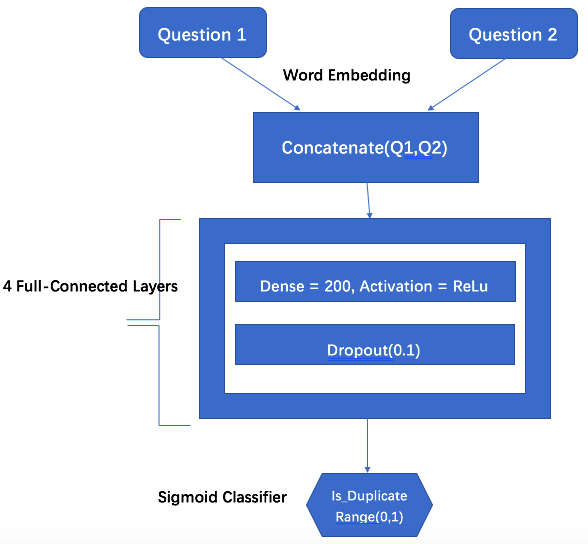
\includegraphics[width = 0.85\textwidth]{figures/modelac.png}
		\caption{Model architecture}
	\end{figure}
	
	we choose the $relu$ activation function because of its performance better than other activation functions in the one hot vector calculation. Also, we determine to use sigmoid as the activation function in the bottom layer because the sigmoid activation function is better for the binary classification problem. Our approach also adopts the Batch normalization algorithm[13] that can faster the learning speed and higher overall accuracy. There are four fully connected layers which dense is 200 and use dropout to overcome the overfitting problem. 
	\par
	For the last layer, the DSSM should output a parameter called is\_duplicate that range from 0 to 1, which indicates the similarity of the input question pair. We use the sigmoid activation function and binary cross entropy for this binary classification problem.
	\par
	